\documentclass{article}

\usepackage[margin=1.0in]{geometry}
\usepackage{graphicx}
\usepackage{amsmath}
\usepackage{float}
\usepackage{enumitem}

\title{CSC 535 HW3}
\date{9/21/2018}
\author{Simon Swenson}

\begin{document}

\pagenumbering{gobble}
\maketitle
\pagenumbering{arabic}

\large Introduction

\small I completed all of the required homework problems and chose problem 7 as 
opposed to problem 8.

\section{Q1}

Recall that expected loss, $ EL = \int L(\Theta, \hat{\Theta}) p(\Theta | X) d 
\Theta $. If our loss function $ L(\Theta, \hat{\Theta}) = (\Theta - \hat{\Theta})^2 $,
we have the expression $ EL = \int (\Theta - \hat{\Theta})^2 p(\Theta | X) d \Theta$.
To minimize this expected loss, we find the derivative and set it to zero to 
find the local minima and maxima:

\begin{align*}
\frac{d EL}{d \hat{\Theta}} &= \frac{d EL}{d \hat{\Theta}} (\int (\Theta - \hat{\Theta})^2 p(\Theta | X) d \Theta) \\
\frac{d EL}{d \hat{\Theta}} &= \int -2 (\Theta - \hat{\Theta}) p(\Theta | X) d \Theta \\
\end{align*}

Let $ \frac{d EL}{d \hat{\Theta}} = 0 $. Then:

\begin{align*}
\int -2 (\Theta - \hat{\Theta}) p(\Theta | X) d \Theta                             &= 0 \\
-2 (\int \Theta p(\Theta | X) d \Theta - \int \hat{\Theta} p(\Theta | X) d \Theta) &= 0 \\
\int \Theta p(\Theta | X) d \Theta                                                 &= \int \hat{\Theta} p(\Theta | X) d \Theta \\
\int \Theta p(\Theta | X) d \Theta                                                 &= \hat{\Theta} \int p(\Theta | X) d \Theta
\end{align*}

Recall that $ \int p(\Theta | X) d \Theta = 1 $

Then $ \int \Theta p(\Theta | X) d \Theta = \hat{\Theta} $. However, we have 
only proven that this is a minimum or maximum. We take the second derivative to 
find concavity:

\begin{align*}
EL'' &= \frac{d}{d \hat{\Theta}}(\int -2(\Theta - \hat{Theta})p(\Theta | X) d \Theta) \\
     &= \frac{d}{d \hat{\Theta}}(-2 \int \Theta p(\Theta | X) d \Theta + 2 \hat{\Theta} \int p(\Theta | X) d \Theta) \\
     &= 2 \int p(\Theta | X) d \Theta \\
     &= 2
\end{align*}

Thus, the function is always concave up, and the extremum that we found earlier 
is a minimum.

\section{Q2}

Oh no. You're asking me to do something creative. I don't know if I can manage 
that.

Suppose that you're in some horror flick and being chased by a crazy mass 
murderer. In such a scenario, you should be quiet. In fact, making too much 
noise will increase the chances of the killer catching you. However, the killer 
has also laid out some traps in the area. Getting caught in a trap could also 
increase the chances of the killer catching you. Our three random variables are 
thus $ A = $ making too much noise, $ B = $ falling prey to one of the killer's 
traps and $ C = $ getting caught by the killer.

Let's say that we've observed $ C $, that is, we've unfortunately been caught. 
Rather than coming up with an escape plan, we've decided to muse on the 
intricacies of probability, as mathematicians are wont to do. If we know that 
we've made too much noise, but don't know anything about whether we fell prey 
to one of the killer's traps (maybe we have amnesia!), we've actually been given some information of 
whether we fell prey to a trap or not. If we were caught and we made 
too much noise, we can intuitively reason that we are less likely to have been 
caught due to a trap than if we didn't know whether we made too much noise or 
not. This is the "explaining away" principle in action.

Let's hypothesize more on this probability distribution in our final moments. 
Consider the following probability distribution. The first table is the table 
when we weren't caught (c = 0), and the second table is the table when we were 
caught (c = 1).

$P(c = 0)$:

\begin{tabular}{r | c c}
               & $P(a = 0)$ & $P(a = 1)$ \\
    $P(b = 0)$ &     0.3575 &     0.0125 \\
    $P(b = 1)$ &     0.0125 &     0.0075
\end{tabular}

~\\
~\\

$P(c = 1)$:

\begin{tabular}{r | c c}
               & $P(a = 0)$ & $P(a = 1)$ \\
    $P(b = 0)$ &       0    &     0.18   \\
    $P(b = 1)$ &       0.28 &     0.1500   
\end{tabular}

To prove that A and B are independent, we can marginalize the other varaibles:

\begin{align*}
P(a = 0) &= 0.65 \\
P(a = 1) &= 0.35 \\
P(b = 0) &= 0.55 \\
P(b = 1) &= 0.45
\end{align*}

Then compare:

\begin{align*}
P(a = 0, b = 0) = 0.3575 = (0.65)(0.55) = P(a = 0)P(b = 0) \\
P(a = 1, b = 0) = 0.1925 = (0.35)(0.55) = P(a = 1)P(b = 0) \\
P(a = 0, b = 1) = 0.2925 = (0.65)(0.45) = P(a = 0)P(b = 1) \\
P(a = 1, b = 1) = 0.1575 = (0.35)(0.45) = P(a = 1)P(b = 1)
\end{align*}

We see that, for all cases, independence holds, so independence between $A, B$ holds.

From there, since we know c = 1, we can take that as a condition and normalize 
the second table:

\begin{tabular}{r | c c}
               & $P(a = 0)$     & $P(a = 1)$ \\
    $P(b = 0)$ & 0              & $\sim 0.29508$ \\
    $P(b = 1)$ & $\sim 0.45902$ & $\sim 0.24590$   
\end{tabular}

Here, we can again compute the probabilities of $a, b$ by marginalizing:

\begin{align*}
P(a = 0) &\approx 0.45902 \\
P(a = 1) &\approx 0.54098 \\
P(b = 0) &\approx 0.29508 \\
P(b = 1) &\approx 0.70492
\end{align*}

We can again compare the joint probabilities against the values if they were 
independent:

$$
P(a = 0, b = 0) = 0 \neq 0.13545 \approx (0.45902)(0.29508) \approx P(a = 0)P(b = 0)
$$

Thus, $ A \bot B $, but $ A \neg \bot B | C $.

\section{Q3}

\begin{figure}[!ht]
	\centering
	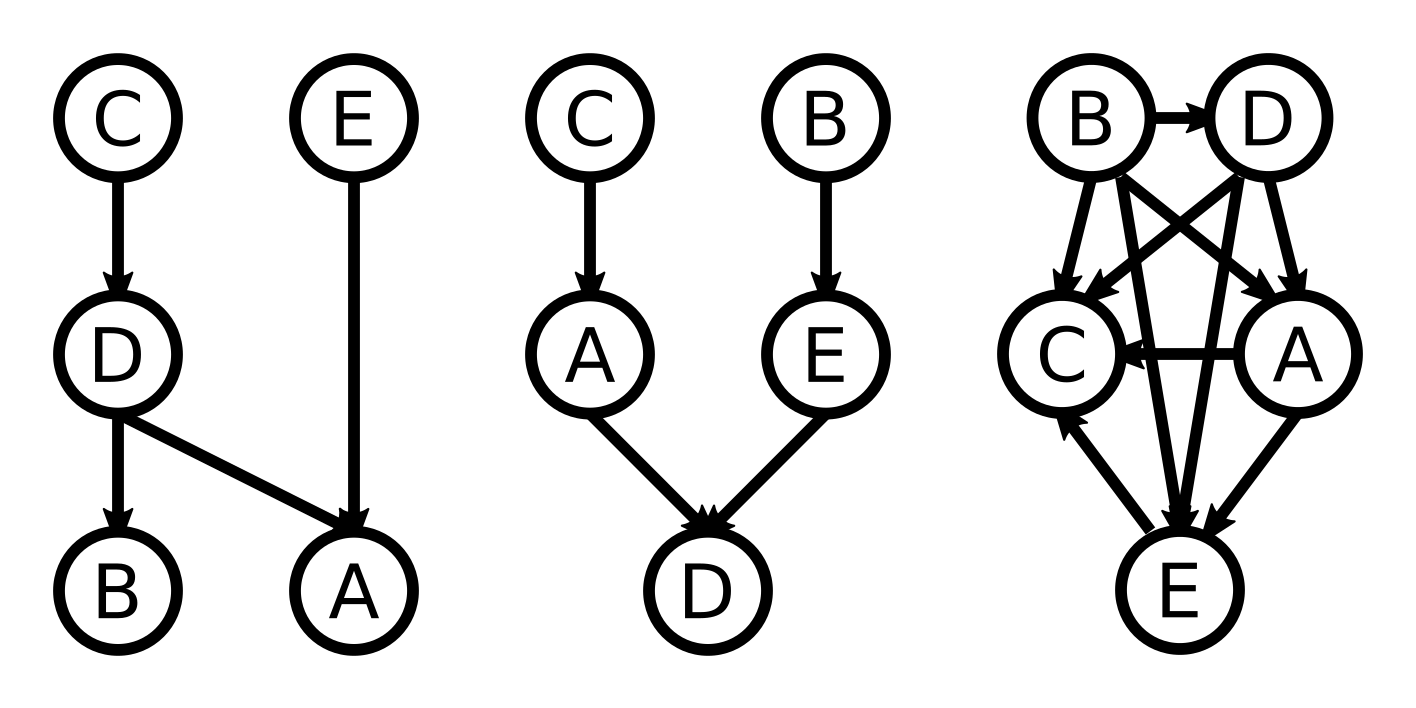
\includegraphics[width=120mm]{q3-all-graphs.png}
	\caption{The three graphs for the three distributions given below. From left to right: the graph for a, the graph for b, and the graph for c.}
\end{figure}

\subsection{a}

Given: $ p(A, B, C, D, E) = p(A | D, E) p(B | D) p(C) p(D | C) p(E) $, we can 
rearrange the factorization:

$$
p(A, B, C, D, E) = p(C) p(D | C) p(B | D) p(E) p(A | D, E)
$$

This is different from the canonical chain rule, highlighting some structural 
differences between the data. By chain rule, the canonical form would be:

$$
p(A, B, C, D, E) = p(C) p(D | C) p(B | C, D) p(E | B, C, D) p(A | B, C, D, E)
$$

As is evident, in the given expression, $B$ is not conditioned on $C$, $E$ is not 
conditioned on anything, and $A$ is not conditioned on $B, C$, whereas the 
canonical chain rule conditions $ B $ on $C$ (in addition to $ D$), $E$ on $B, C, D$, 
and $A$ on $B, C$ (in addition to $D, E$).

\subsection{b}

Given: $ p(A, B, C, D, E) = p(A | C) p(E | B) p(C) p(B) p(D | A, E) $, we can 
rearrange the factorization:

$$
p(A, B, C, D, E) = p(C) p(A | C) p(B) p(E | B) p(D | A, E)
$$

There are also substatial differences between this expression and the 
expression achieved from the canonical chain rule:

$$
p(A, B, C, D, E) = p(C) p(A | C) p(B | A, C) p(E | A, B, C) p(D | A, B, C, E)
$$

In particular, we see that, in the original expression, neither $B$ nor $E$ are 
conditioned on $A, C$. In addition, $D$ is not conditioned on $B, C$.

\subsection{c}

Given: $ p(A, B, C, D, E) = p(C | A, B, D, E) p(A | B, D) p(D | B) p(B) p(E | A, B, D) $, 
we can rearrange the factorization:

$$
p(A, B, C, D, E) = p(B) p(D | B) p(A | B, D) p(E | A, B, D) p(C | A, B, D, E)
$$

Unlike the previous two expressions, this expression is actually isomorphic 
to the canonical chain rule. In addition, the demonic summoning circle 
represented in the graph is a good parallel for how little information the 
canonical chain rule actually gives us. Like summoning demons to this realm, 
using the canonical chain rule should be avoided, if possible. In particular, 
we should use priors, if we have any, about which variables affect which other 
variables.

(Hopefully the humor wasn't too over the top.)

\section{Q4}

Recall the process for d-separation:

\begin{itemize}
    \item Set all condition nodes to observed.
    \item For each path connecting the two nodes that we are considering independence for:
    \begin{itemize}
        \item For each triple in the path, if that triple signifies independence, 
            then mark this path as broken.
    \end{itemize}
    \item If all paths are broken, denote independence. Otherwise, we cannot say.
\end{itemize}

\subsection{a}

\subsubsection{C independent of B given D}

First, we observe/mark D. Then, we consider all paths connecting C and B. Only one 
such path exists: $C \rightarrow D \rightarrow B$. This is a chain with the 
center (D) observed. Therefore, this path is broken, and $C \bot B | D$

\subsubsection{E independent of C given B}

First, we observe/mark B. Then, we consider all paths connecting E and C. There 
is only one such path: $ C \rightarrow D \rightarrow A \leftarrow E $. 
$C \rightarrow D \rightarrow A$ is a chain with D unobserved, and is thus 
unbroken. $ D \rightarrow A \leftarrow E $ is a V with A unobserved. Therefore, 
the chain is broken, and $ E \bot C | B $.

\subsection{b}

\subsubsection{C independent of B given D}

First, we observe/mark D. Then, we consider all paths connecting C and B. Only one 
such path exists: $ C \rightarrow A \rightarrow D \leftarrow E \leftarrow B $. 
$ C \rightarrow A \rightarrow D $ is a chain with A unobserved, which does not break this path.
$ A \rightarrow D \leftarrow E $ is a v with D observed, which does not break this path. 
$ D \leftarrow E \leftarrow B $ is a chain with E unobserved, which does not break this path.
Thus, C is not necessarily conditionally independent of B, given D.

\subsubsection{E independent of C given B}

First, we observe/mark B. Then, we consider all paths connecting E and C. Only one 
such path exists: $ C \rightarrow A \rightarrow D \leftarrow E $. 
Check $ C \rightarrow A \rightarrow D $, a chain with A unobserved, thus path unbroken.
Check $ A \rightarrow D \leftarrow E $, a v with D unobserved. This breaks the path, so 
$ E \bot C | B $.

\subsection{c}

\subsubsection{C independent of B given D}

First, we observe/mark D. Then, we would normally consider all paths connecting 
C and B. However, Since there exists a two-node path $ B \rightarrow C $, which 
cannot be broken, we can immediately conclude that we cannot say that C is 
independent of B, given D, with just the graph structure.

\subsubsection{E independent of C given B}

This is similar to above. Since there exists a two-node path $ E \rightarrow C $, 
which cannot be broken, we can immedately conclude that we cannot say that E is 
independent of C, given B.

\section{Q5}

\subsection{a}

\begin{figure}[!ht]
	\centering
	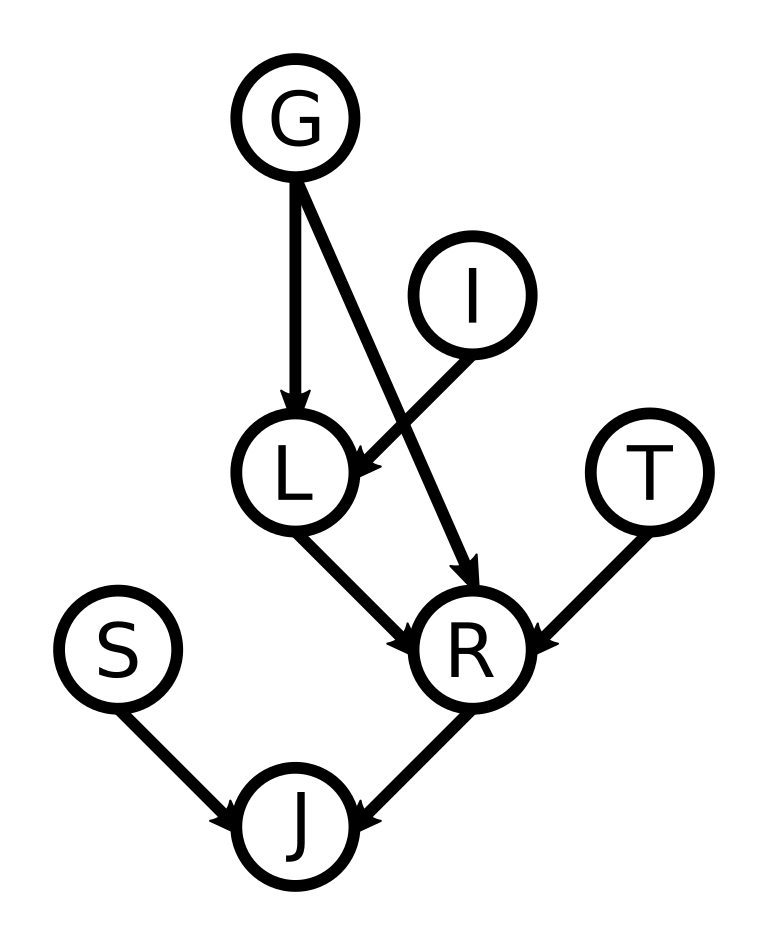
\includegraphics[width=60mm]{q5-graph.png}
	\caption{The influence of various factors on your long-term academic 
        prospects. 
        G = grades, 
        I = interactions with your letter-writing professors, 
        L = letters of recommendation from those professors, 
        T = GRE test scores, 
        R = rank of the graduate program you get into, 
        S = state, 
        J = academic job}
\end{figure}

\subsection{b}

$$
P(G, I, L, T, R, S, J) = P(G) P(I) P(L | G, I) P(T) P(R | G, L, T) P(S) P(J | R, S)
$$

\subsection{c}

We can use the "alternative Bayesian network semantics" here. $NonDescendents(J) = \{G, I, L, T, R, S\}, Parents(J) = \{S, R\}$. 
Since $G \in NonDescendents(J) \wedge R \in Parents(J) $, $J \bot G | R$. In laymen's terms, Knowing your college rank blocks grades 
from job.

\subsection{d}

GRE scores \textit{are} independent of grades in this model. We can use d-separation to prove it.
There are two paths: $ G \rightarrow R \leftarrow T $ and $ G \rightarrow L \rightarrow R \leftarrow T $. 
Both include a v with an unobserved center node ($ L \rightarrow R \leftarrow T $ and $ G \rightarrow R \leftarrow T $). 
Thus, both are blocked.

\subsection{e}

GRE scores \textit{are} independent of the letter of recommendation in this model. Again, we can use d-separation. 
There are again two paths: $ L \rightarrow R \leftarrow T $ and $ L \leftarrow G \rightarrow R \leftarrow T $. 
The same two triples as in d block here, as well: $ L \rightarrow R \leftarrow T $ and $ G \rightarrow R \leftarrow T $.

\subsection{f}

Now that we are conditioning on the rank of the grad program, everything changes. 
As those v nodes were the only blocking nodes, conditioning on R causes them to 
no longer block. Therefore, the GRE scores are not independent of the letter of 
recommendation, conditioned on the rank of the graduate program.

\subsection{g}

Consider the path $ G \rightarrow R \leftarrow L \leftarrow I \rightarrow J $. 
Since R is observed, $ G \rightarrow R \leftarrow L $ is unblocked. Furthermore, 
neither L nor I are observed, so $ R \leftarrow L \leftarrow I $ is unblocked and 
$ L \leftarrow I \rightarrow J $ is unblocked. Therefore, since there is a 
completely unblocked path, we can no longer conclude that G is independent of J, 
given R.

In plain English, since we know the rank of the graduate program attended, knowing 
the grades gives us some information about the quality of the letter of recommendation. 
For example, if the rank of the graduate program is very high, but the student got 
poor grades, he or she is more likely to have had an excellent letter of recommendation.
This information of the letter of recommendation gives us some info about the student's 
relationship with his or her instructor. Finally, that relationship with his or 
her instructor directly influences whether he or she got the job.

\subsection{h}

The two are still not necessarily independent, given the conditions. Consider the 
path $ G \rightarrow L \leftarrow I \rightarrow J $. Specifically, the triple 
$ G \rightarrow L \leftarrow I $ is unblocked, since L is now observed.

In plain english, since we know the letter of recommendation, knowing grades could 
give us some information on the student's interactions with instructors. For example, 
if the student got very poor grades but received an excellent letter of recommendation, 
he or she probably had steller interactions with his or her instructors. Finally, 
those interactions with instructors will directly influence whether the student 
got a job.

\section{Q6}

\subsection{d}

Using alternative bayesian network semantics:

\begin{itemize}
    \item Consider node A. $NonDescendents(A) = \{B\} \wedge Parents(A) = \emptyset$, so $ A \bot B $.
    \item Consider node B. Symmetric to A.
    \item Consider node C. $NonDescendents(C) = \emptyset \wedge Parents(C) = \{A, B\}$, so C has no conditional independence relationships.
    \item Consider node D. $NonDescendents(D) = \{A, B, E, F\} \wedge Parents(D) = \{C\}$, so $D \bot \{A, B, E, F\} | \{C\}$.
    \item Consider node E. $NonDescendents(E) = \{A, B, D\} \wedge Parents(E) = \{C\}$, so $E \bot \{A, B, D\} | \{C\}$.
    \item Consider node F. $NonDescendents(F) = \{A, B, C, D\} \wedge Parents(F) = \{E\}$, so $F \bot \{A, B, C, D\} | \{E\}$.
\end{itemize}

\subsection{e}

\begin{align*}
P(A, B, C, D, E, F) &= P(A) P(B | A) P(C | A, B) P(D | A, B, C) P(E | A, B, C, D) P(F | A, B, C, D, E) \\
                    &= P(A) P(B) P(C | A, B) P(D | A, B, C) P(E | A, B, C, D) P(F | A, B, C, D, E) \\
                    &= P(A) P(B) P(C | A, B) P(D | C) P(E | A, B, C, D) P(F | A, B, C, D, E) \\
                    &= P(A) P(B) P(C | A, B) P(D | C) P(E | C) P(F | A, B, C, D, E) \\
                    &= P(A) P(B) P(C | A, B) P(D | C) P(E | C) P(F | E)
\end{align*}

\subsection{f}

$$
P(A, B, C, D, E, F) = P(A) P(B) P(C | A, B) P(D | C) P(E | C) P(F | E)
$$

It is the same, as was expected. However, this is because we chose a convenient 
order for the chain rule. However, since we \textit{can} choose an order arbitrarily, 
this doesn't invalidate the reasoning: The equivalence shows that the two ways of thinking about 
Bayes nets are equivalent.

\section{Q7}

\begin{figure}[!ht]
	\centering
	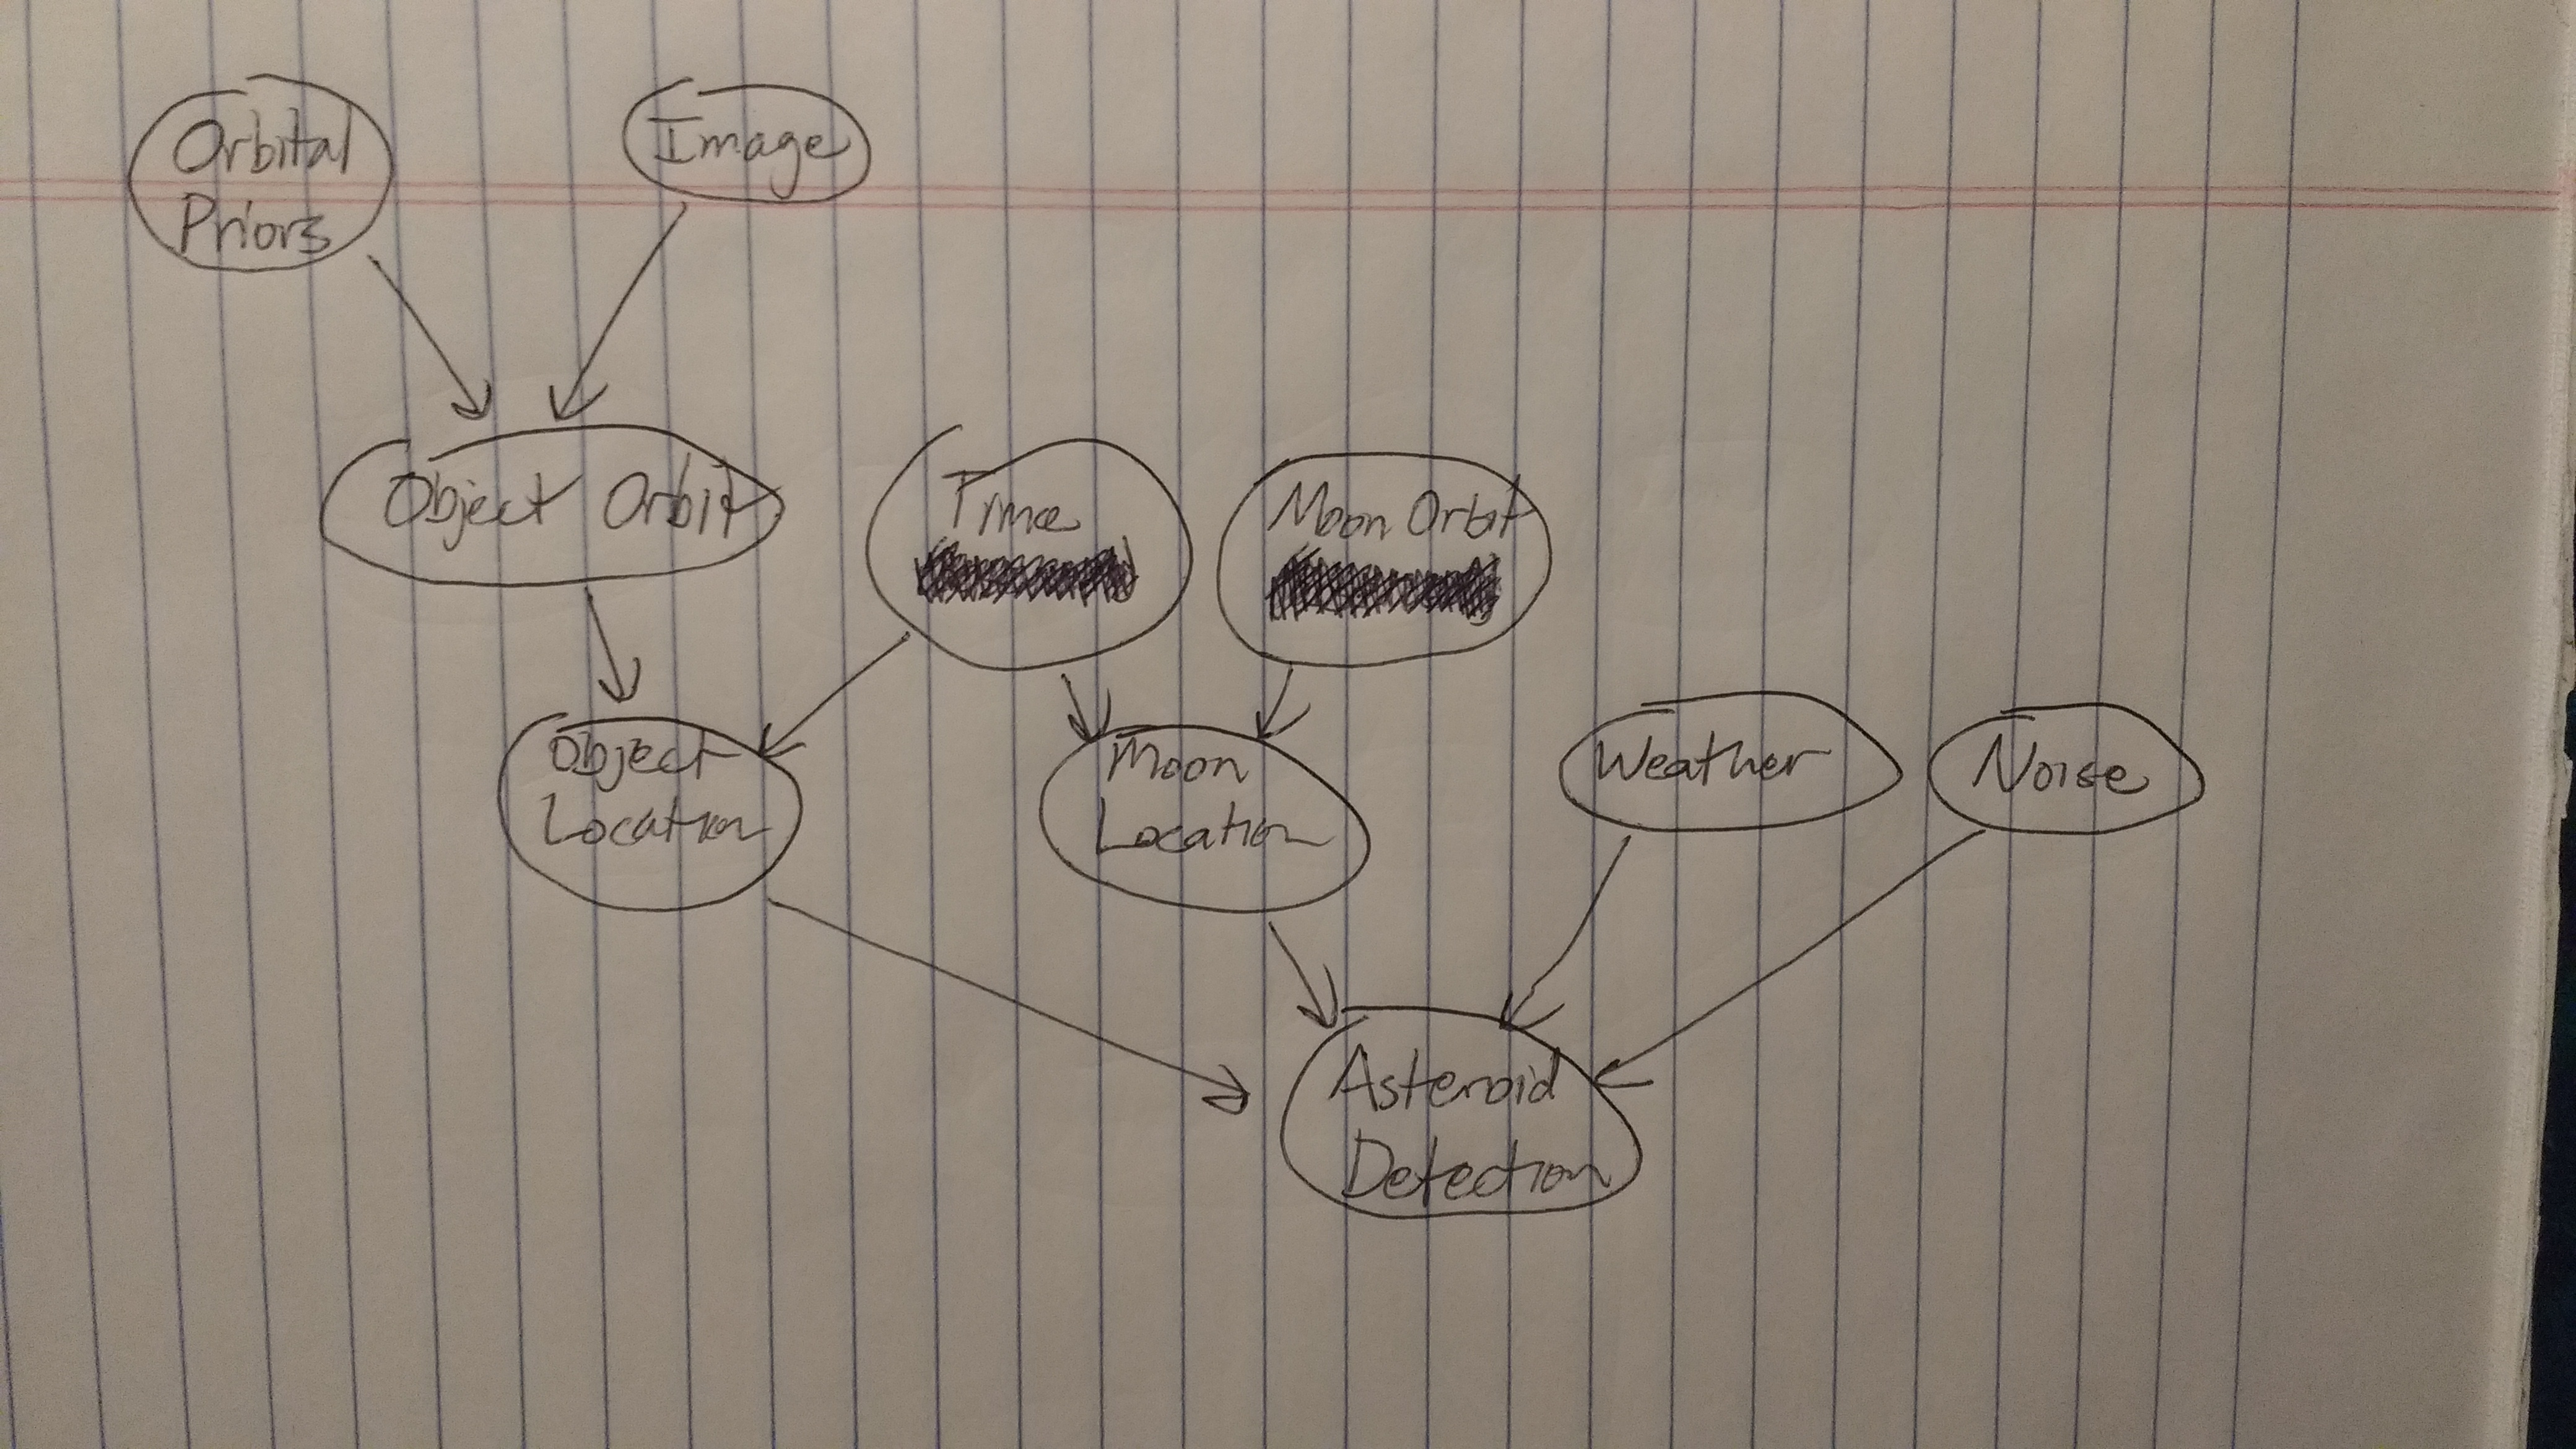
\includegraphics[width=120mm]{q7-graph.jpg}
	\caption{The influence of various factors on whether an asteroid was detected 
        or not.}
\end{figure}

As can be seen in the graph, there are eight random variables:

\begin{itemize}
    \item Orbital Priors
    \item Image
    \item Object Orbit
    \item Time
    \item Object Location
    \item Moon Orbit
    \item Moon Location
    \item Weather
    \item Random Hallucinations
\end{itemize}

Based on the description, there is a lot at play when determining the detector's 
end judgment. Several variables are easily dealt with, such as weather, noise, 
and the moon's location. We are not really given much more information about these 
variables, so those are somewhat dead ends. However, we can infer the moon's 
location similar to how we infer an object's location by taking its known orbit 
and the time annotation into account. The last random variable which factors into 
asteroid detection is the object's location, itself. This is a bit more complicated. 
We are given that we can find the object's location, given its orbit and the time, 
so ensure that the object's location depends on those two variables. However, the 
object's orbit can be further broken down. Recall that we have an image we are 
considering. Assume we have an object detection algorithm that can mark an object 
in an image. Then, that mark in the image, along with the orbital priors, can 
determine the object's orbit.

Generating a sample is an extension of the sampling method outlined by Clay 
several weeks ago. Each random variable has a probability density (or mass, for 
discrete distributions) function associated with it. We 
start at the top of the graph. Thus, we first generate an image based on the 
probability density function of that image. (This may be complicated, and may 
even break into more nodes.) Then, we use our orbital priors along with that image 
as priors for the object's orbit, using the same sampling method as before, but 
taking the image and the orbital priors into account. We then randomly sample time 
from the time distribution. If we have a good amount of training data, we may be 
able to determine this distribution fairly easily. Then, we generate the object's 
location from the location distribution, given the object's orbit and the time. 
We know the moon's orbit, so we can generate the moon's location from the time 
and the moon's orbit by using the moon location PDF. Finally, we can randomly 
generate weather and noise variables, all factoring into the asteroid detection 
distribution, which we can now generate, knowing the priors.

\end{document}